In this chapter, we show two instances of encoding textual inputs in the context of external knowledge. The first model shown here is an ontology-aware recurrent neural network, an encoder that has access to the token level semantic information from an ontology (Wordnet).
Despite their empirical success, type-level word embeddings ignore the semantic ambiguity of lexical items. We address this problem by using Wordnet to find the collection of semantic concepts manifested by a word type, and represent a word type as a collection of concept embeddings. We show
how to integrate the proposed ontology-aware lexical representation with recurrent neural networks (RNNs) to model token sequences. The second model is proposed 

\section{Ontology Aware Recurrent Neural Networks}
A human can process new information in a sentence, use context to resolve ambiguities, and use commonsense to make relevant generalizations.
For instance, when Alice tells Bob \textit{``Children and parents are splashing water at the pool,''} Bob may reasonably expect that Alice means the `swimming pool' sense of the word `pool' and also infer that \textit{``Children are playing outside with adult supervision.''}
In contrast, semantic ambiguity and commonsense inference constitute major challenges for computational models of language \citep{yarowsky:94,tanaka:07,celikyilmaz:13,pasca:14}.
Computational models used for machine reading (e.g., \cite{bowman:15}) often use the same representation for all instantiations of a word type, ignoring semantic ambiguity at the lexical level.  We focus on word embeddings as an important component of many computational models of language.
Type-level word embeddings are a lexical representation which maps a word type (i.e., a surface form)\footnote{We use the term `word type' to refer to the surface form of a word, and the term `word token' to refer to a particular instantiation of the word in text.} 
to a dense vector of real numbers such that similar word types have similar embeddings. 
Despite their empirical success (e.g. \cite{socher:10}) they inherently ignore the semantic ambiguity of word types (e.g., `pool' may refer to a swimming pool or the pocket billiards sport)  and do not explicitly model lexical generalizations (e.g., a swimming pool is a container).

The model proposed here uses WordNet \citep{miller1995wordnet} to encode generalizations and semantic ambiguity in computational models at the lexical level.\footnote{Other resources which specify relationships between lexical items (e.g., FrameNet) may also be used.}
WordNet groups synonymous words into synsets (i.e., concepts), with polysemous words belonging to different synsets. Synsets have multiple labeled relations among them, and in this paper, we focus on the hypernymy relation which defines a hierarchy of lexical generalizations.
For example, the word \textit{pool} belongs to nine different synsets (e.g., swimming pool, collection of things, pocket billiards).
\footnote{Unlike the examples listed here, the distinctions between some synsets in WordNet are very specific. For example, one of the nine synsets for \textit{pool} is defined as ``a communal combination of funds.''}
For example, the direct hypernym of the pocket billiards sense of \textit{pool} is \textit{table game}.
The hypernym paths are different for different senses of the word, with some hypernyms shared among senses.

We map each word type to a grid of concept embeddings (see Fig.~\ref{fig:ontolstm_tensor}), which are shared across many words. The word representation is computed as a distribution over the concept embeddings from the word's grid. We show how these distributions can be 
learned conditioned on the context when the representations are plugged into RNNs.
Intuitively, commonsense knowledge encoded as WordNet relations could potentially help with language understanding tasks. 
but mapping tokens to entities in WordNet is a challenge. One needs to at least disambiguate the sense of the token before being able to use the relevant information. Similarly, not all the hypernyms defined by WordNet may be useful for the task at hand as some may be too general to be informative.
 
\begin{figure}[t]
\begin{center}
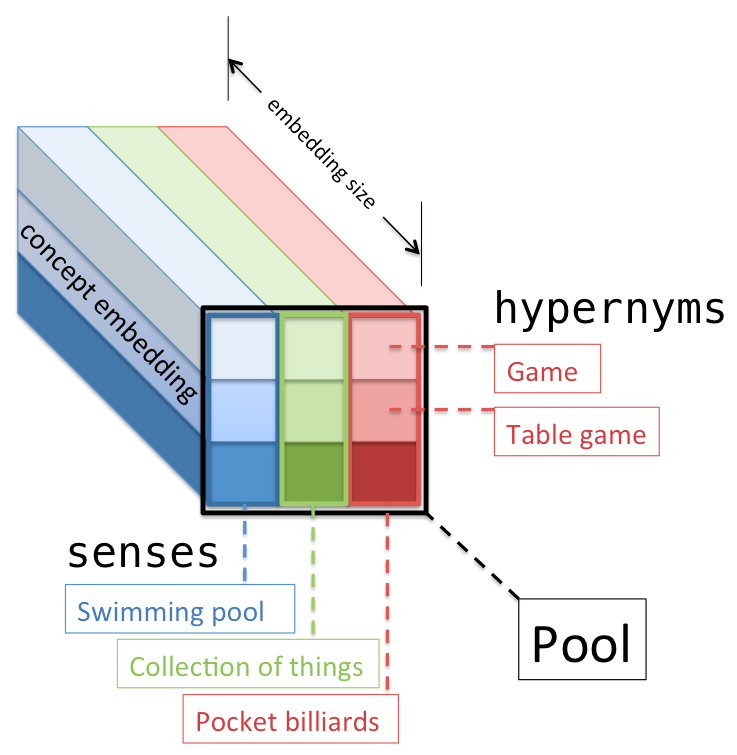
\includegraphics[width=3in]{figures/tensor2.png}
\caption{Example of ontology-aware lexical representation}
\label{fig:ontolstm_tensor}
\end{center}
\end{figure}

\subsection{Related Work}
% concept embeddings
Previous work used lexical ontologies such as WordNet to improve \textit{pretrained} word embeddings at the \textit{type level}.
\cite{yu:14} extended the CBOW model \citep{mikolov:13} by adding an extra term in the training objective for generating words conditioned on similar words according to a lexicon.
\cite{jauhar:15} extended the skipgram model \citep{mikolov:13} by representing word senses as latent variables in the generation process, and used a structured prior based on the ontology.
\cite{faruqui:15} used belief propagation to update pretrained word embeddings on a graph that encodes lexical relationships in the ontology.
In contrast, we propose an approach for obtaining \textit{context-sensitive} embeddings at the token level, while \textit{jointly} optimizing the model parameters for the NLP task of interest.
Previous work used WordNet and other lexical resources such as the paraphrase database of \cite{ganitkevitch:13} to improve type-level word embeddings.
Related to the idea of concept embeddings is \cite{rothe:15} who estimated WordNet synset representations, given pretrained type-level word embeddings.
 In contrast, our work focuses on estimating token-level word embeddings given concept embeddings.
 Related to token-level embeddings is \cite{belanger:15} who proposed a Gaussian linear dynamical system for estimating token-level word embeddings. However, this approach does not make use of lexical ontologies and is not amenable for joint training with a downstream NLP task.

\subsection{Ontology-aware Recurrent Neural Networks}
\subsubsection{Lexical Representation}
\label{sec:ontolstm_input_rep}
To address the semantic ambiguity in traditional word embeddings, we represent each word type as a grid of concept embeddings, organized in a third-order tensor (i.e., a 3-dimensional array), as shown in Fig.~\ref{fig:ontolstm_tensor}, 
which is an example for the word \textit{pool}. The three dimensions correspond to senses, hypernyms per sense, and dimensionality of the synset embeddings respectively. We emphasize that synset embeddings have one-to-one correspondence with WordNet synsets,
and are shared across the tensor representation of multiple word types.

We use $T_w$ to denote the third-order tensor representation of a word $w$.
and $T_w(s,y)$ to refer to the $d$-dimensional concept embedding in the tensor which corresponds to a word sense $s$ and a hypernym $y$; e.g., $T_{\text{pool}}(\text{Pocket billiards},\text{Table game})$.
Other words share the same concept embedding, such as $T_{\text{dominoes}}(\text{dominoes game},\text{Table game}) = T_{\text{pool}}(\text{Pocket billiards},\text{Table game})$.
We truncate the tensor or pad it with zeros as needed, since different word types have different numbers of word senses, and different synsets have different numbers of hypernyms. 
With $S$ denoting a predefined, fixed number of senses per word type and $Y$ denoting a predefined, fixed number of generalizations (i.e., number of hypernyms plus one) per word sense, all tensor embeddings are of the same size: $T_w \in \mathbb{R}^{S\times Y \times d}$.
Unlike type-level representations in the proposed setup, rare words can leverage the concept embedding parameters shared with other words close to them in the WordNet graph structure.

\subsubsection{Ontology-Aware LSTM (OntoLSTM)}
\label{sec:ontolstm}
Recurrent Neural Networks (RNN) model sequences by repeating the same neural network module (i.e., the same model parameters) for each position in the sequence.
RNNs have been widely used for several NLP tasks, including language modeling \citep{mikolov:10}, textual entailment \citep{bowman:15}, speech recognition \citep{graves:13}, machine translation \citep{sutskever:14} and dependency parsing \citep{dyer:15}.
We now show how to use this lexical representation for modeling sequences by plugging them into long short-term memory networks  (LSTM, \cite{hochreiter1997long}) a popular type of RNNs.
At position $t$, the LSTM consumes the previous hidden state of the sequence $h_{t-1}$ and a vector representation of the input word at this position $i_t$, and produces the current hidden state $h_t$.\footnote{The interface of LSTM modules also includes a cell state which runs down the sequence with only minor linear transformations.}
Instead of using type-level word embeddings to represent the input at each position, we consider using token-level, ontology-aware word embeddings.
\begin{figure}
  \begin{center}
  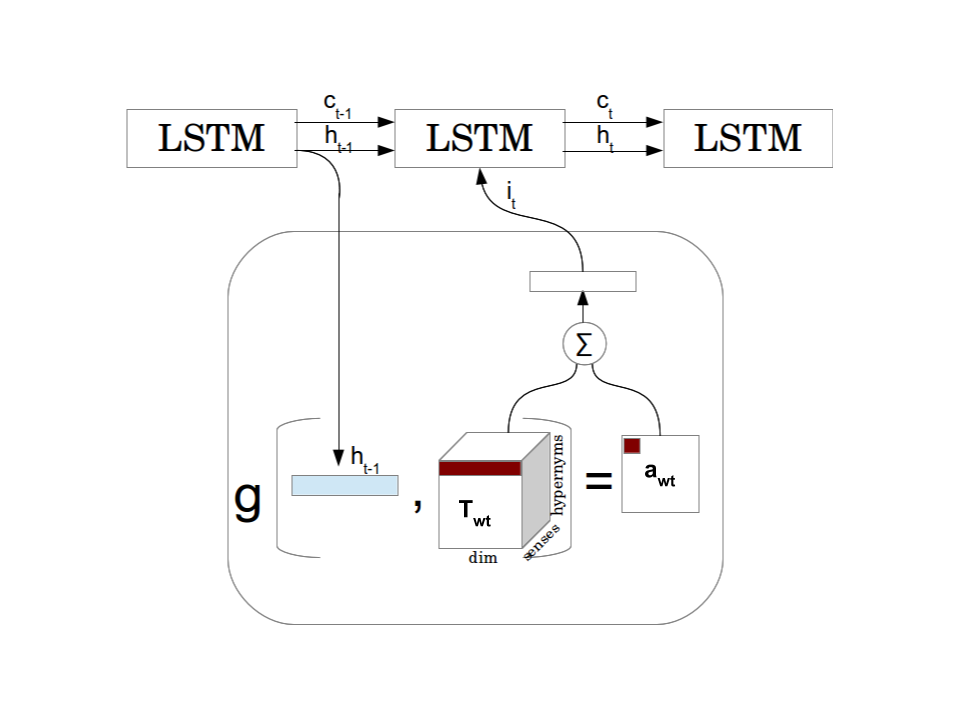
\includegraphics[width=5in]{figures/ontolstm_diagram_modified.png}
  \caption{Schematic of OntoLSTM}
  \label{fig:ontolstm_model}
  \end{center}
 \end{figure}

The modification we propose is specific to the representation of input words ($i_t$). 
At each position $t$, we dynamically compute $i_t$ (corresponding to the token $w_t$) as a function of (a) the concept embeddings in $T_{w_t}$ and (b) the output of the previous timestep $h_{t-1}$, as shown in Figure~\ref{fig:ontolstm_model}.
Precisely, $i_t = \mathbb{E}_{p(s,y\mid w_t, h_{t-1})}\big[ T_{w_t}(s,y) \big]$ is the expected value of relevant concept embeddings, according to a discrete probability distribution over senses $s$ and hypernyms $y$.

\paragraph{Uniform attention:} The first variant of our model defines a uniform distribution for $p(s,y \mid w_t, h_{t-1})$. That is, we take a simple average of the synset embeddings in the grid to get the word representation. We call this variant \textbf{$\text{OntoLSTM}_{\text{uni}}$}.

\paragraph{Parameterized attention:}
The second variant of the model learns to weigh hypernyms differently conditioned on the context.
Although attention mechanisms are typically used to explicitly represent the importance of each item in a sequence \citep{bahdanau:14}, the can also be applied to non-sequential items.

We calculate an attention score for each generalization of each word sense in the following way:
\begin{equation}
\begin{aligned}[c]
M_t^y &= \tanh(T_{w_t}W_i^y + (\mathbbm{1}_{S \times Y}\otimes h_{t-1}) W_h^y) \nonumber \\
a_t^y &= \mathrm{softmax}(M_t^y q, 2) \nonumber \\
\end{aligned}
\begin{aligned}
&\in \mathbb{R}^{S\times Y \times l} \\
&\in \mathbb{R}^{S\times Y} \\
\end{aligned}
\end{equation}
where $(\mathbbm{1}_{S \times Y}\otimes h_{t-1}) \in \mathbb{R}^{S \times Y \times d}$ replicates the hidden state one time for each (word sense, generalization) pair then multiplies $W_h^y \in \mathbb{R}^{d \times l}$ producing $M_t^y \in \mathbb{R}^{S\times Y \times l}$. $W_i^y \in \mathbb{R}^{d \times l}$, $W_h^y \in \mathbb{R}^{d \times l}$ and scoring operator $q \in \mathbb{R}^l$ are model parameters. $\mathrm{softmax}(A,2)$ applies the softmax operation along the second dimension so that the attention scores of all generalizations of a word sense sum to one. Intuitively, $M_t^s$ computes a dense vector representation of length $l$ for each word sense, which is then multiplied by $p$ and normalized to compute the attention scores $a_t^s$. Similarly, $M_t^y$ operates on each (word sense, generalization) pair, and $q \in \mathbb{R}^l$ and gives hypernym attention $a_t^y$.

\paragraph{Sense Priors}: WordNet organizes senses of a word in the order of their frequency (i.e.the first sense of any word is its most frequent sense). We account for this property of the ontology by setting a prior on the sense probability. Precisely,
\begin{equation*}
    p(s|w_t) \sim \text{Exponential}(\lambda_{w_t})
\end{equation*}
We define one rate parameter $\lambda_{w_t}$ per each word type.

Finally, $i_t$ is computed as:
\begin{align}
%i_t &= \mathds{E}_{p(s,y\mid w_t, h_{t-1})}\big[ T_{w_t}(s,y) \big] \nonumber \\
i_t &= \sum_{s, y} p(s|w_t) \times a_t^y(s,y) \times T_{w_t}(s,y) \nonumber
\end{align}
We call this variant \textbf{$\text{OntoLSTM}_{\text{att}}$}.
%Note that the number of input representation parameters in both variants of OntoLSTM is not significantly higher than that of the LSTM. This is because the vocabulary sizes are comparable in both models, and tensors in OntoLSTM share many of the same synset representations.

\subsection{Experiments}
\label{sec:ontolstm_experiments}
We evaluate our model on the natural language inference task.
We show that $\text{OntoLSTM}_{\text{uni}}$ and $\text{OntoLSTM}_{\text{att}}$ improve the test set accuracy of the LSTM baseline by 1.9 and 1.8 absolute points, respectively.

\paragraph{Data preprocessing:} The datasets are part-of-speech (POS) tagged using Stanford's POS tagger \citep{toutanova:03}.
To construct the tensor representation, we map the POS-tagged word to the first two synsets in WordNet (i.e. $S=2$), and extract the most direct five hypernyms (i.e., $H=5$). When a synset has multiple hypernym paths, we use the shortest one. In preliminary experiments, we found that using more word senses or more hypernyms per word sense does not improve the performance.
Words which do not appear in WordNet are assumed to have one unique synset per word type with no hypernyms.

% \subsection{Language Modeling}
% \label{sec:lm}

% Here, we use a language modeling task to compare the three RNN models: LSTM, $\text{OntoLSTM}_\text{uni}$ and $\text{OntoLSTM}_\text{att}$.

% %\wacomment{People wanted to know what the SOTA in LM is. We should add citations to support comparing against LSTM. It would be nice if we can show that existing models have test PPL in the same ballpark as our baseline.}


% \paragraph{Setup:}
% All three models predict the next word in a sequence using a tree-factored softmax \cite{baltescu2014pragmatic}.
% The models are trained to maximize log-likelihood of training data, using stochastic gradient descent with early stopping (up to twenty epochs).
% We use train, development and test splits of sizes 18 million, 2 million and 2 million words, respectively, from the Associated Press newswire data in the 3rd edition of the English Gigaword. The vocabulary during training is initialized with words from training and test sets, so all three models have the same vocabulary with no out of vocabulary words.
% \pdcomment{This will change. Results with word and synset singletons in training data replaced with UNK coming soon.}
% All hidden layers, word embeddings and concept embeddings are of size 50.

% %Our models are capable of computing embeddings for words not seen in training by leveraging the underlying concept embeddings shared with other words seen in training.
% %To illustrate this important feature, we provide a breakdown of the perplexities for seen and unseen words (in training), using a fixed vocabulary which includes all words in the train, development and test data splits.
% %\wacomment{Chris, please review this paragraph.}

% \begin{table}
%     \centering
%     \begin{tabular}{|r|r|r|}
%     \hline
%     \textbf{Model} & Train PPL & Test PPL\\
%     \hline
%     LSTM & 258.8 & 264.0\\
%     $\text{OntoLSTM}_{\text{uni}}$ & 159.1 & 160.4\\
%     $\text{OntoLSTM}_{\text{att}}$ & 156.4 & 156.3\\
%     \hline
%     \end{tabular}
%     \caption{Language model perplexities (lower is better) of the train and test splits with three models. $\text{OntoLSTM}_{\text{uni}}$ and $\text{OntoLSTM}_{\text{att}}$ improve the test set perplexity of the LSTM baseline by 39.2\% and 40.7\%, respectively.}
%     \label{tab:lm_results}
% \end{table}

\begin{table}
    \centering
    \begin{tabular}{|l|c|c|c|}
    \hline
    \textbf{Model} & \textbf{Pretrained } & \textbf{Train} & \textbf{Test}\\
    \hline
    Our LSTM                        & No &  &  \\
    $\text{OntoLSTM}_{\text{uni}}$  & No &  &  \\
    $\text{OntoLSTM}_{\text{att}}$  & No &  &  \\ \hline
    LSTM & Yes &   &  \\
    \hline
    \end{tabular}
    \caption{Results on the SNLI dataset. The numbers are accuracies in percentages. Bottom row shows the results reported by \cite{bowman2016fast} using GloVe vectors to represent words.}
    \label{tab:ontolstm_snli_results}
\end{table}
% \paragraph{Results:}
% Table~\ref{tab:lm_results} reports perplexities (lower is better) of the train and test data splits using each of the three language models.
% The $\text{OntoLSTM}_\text{uni}$ model achieves 38\% and 39\% reduction in perplexities of the train and test data splits, respectively.
% %The $\text{OntoLSTM}_\text{uni}$ \wacomment{\ldots}

%\wacomment{volkan:I am not use but this dataset is not standard for LM testing. People usually use 1B word benchmark and PTB (although PTB is not big enough for LM testing). I would go for 1B word benchmark since there are plenty of results on that dataset.}
%\wacomment{volkan: it is important to see the effect of word embedding. I would love to see i) fixed embedding training with glove initialization ii) learning embeddings from scratch (what you reported) iii) finetuning glove with your model. I bet your code is in theano/keras. I can show you how to do finetuning if you need any help. waleed: honestly, i don't think this actually important given the time constraints.}

% \subsection{Natural Language Inference}
% \label{sec:textual_entailment}

%\wacomment{volkan:table-2 should definitely have sota results from bowman et. al. 2006 in bottom row}

% Here, we use a natural language inference task (also known as recognizing textual entailment) to compare the three RNN-based models: LSTM, $\text{LSTM}_\text{uni}$ and $\text{LSTM}_\text{att}$.

\paragraph{Task:}
Given a pair of sentences (premise and hypothesis), the model predicts one of three possible relationships between the two sentences: \textit{entailment}, \textit{contradiction} or \textit{neutral}.
We use the standard train, development and test splits of the SNLI corpus, which consists of 549K, 10K and 10K labeled sentence pairs, respectively.
For example, the following sentence pair is labeled \textit{entailment}:
 \begin{itemize}
  \item \textbf{Premise} \textit{Children and parents are splashing water at the pool.}
  \item \textbf{Hypothesis} \textit{Families are playing outside.}
 \end{itemize}
\paragraph{Model:}
The three models we compare use the same architecture, except for the representation of input tokens.
Following \cite{mou2015recognizing}, we use two LSTM with tied parameters to read the premise and the hypothesis of each example, then compute the vector $h$ which summarizes the sentence pair as the concatenation:
$$h=\big[h_{\text{pre}}; h_{\text{hyp}}; h_{\text{pre}} -h_{\text{hyp}};h_{\text{pre}} *h_{\text{hyp}}\big]$$
where $h_\text{pre}$ is the output hidden layer at the end of the premise token sequence, $h_\text{hyp}$ is the output hidden layer at the end of the hypothesis token sequence.
The summary $h$ then feeds into two fully connected ReLU layers of size 1024, followed by a softmax layer of size 3 to predict the label.
The word embeddings and concept embeddings are of size 300, and the hidden layers 150.
The models are trained to maximize log-likelihood of correct labels in the training data, using ADAM \citep{kingma2014adam} with early stopping (up to twenty epochs).

\paragraph{Results:}
Table~\ref{tab:ontolstm_snli_results} shows the classification results. We also report previously published results of a similar neural architecture as an extra baseline: the 300-dimensional LSTM RNN encoder model in \cite{bowman2016fast}.\footnote{We note this is not the best model presented in \cite{bowman2016fast}, but it is the one that is most similar to our neural architecture.}
They use GloVe as pretrained word embeddings while we jointly learn word/concept embeddings in the same model.
\cite{bowman2016fast}'s LSTM outperforms our LSTM model by 1.5 absolute points on the test set. This may be due to the difference in input representations. Since we learn the synset representations in OntoLSTM, comparison with our LSTM implementations is more sensible.
The $\text{OntoLSTM}_{\text{uni}}$ outperforms the LSTM model with 1.8 absolute points on the test set, illustrating the utility of the ontology-aware word representations in a controlled experiment.

\subsection{Analysis}
\label{sec:discussion}
\begin{figure}
\begin{center}
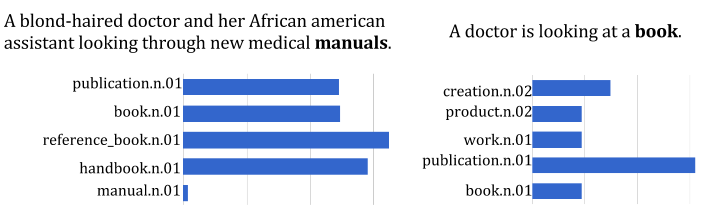
\includegraphics[width=5in]{figures/ontolstm_snli_comparison.png}
\caption{Relative attention values for words in the premise and in the hypothesis.}
\label{fig:snli_visualization}
\end{center}
\end{figure}

\paragraph{Generalization attention:} \label{sec:generalization}
Fig.~\ref{fig:snli_visualization} shows one example from the test set of the SNLI dataset where hypernymy information is useful. 
The LSTM model shares no parameters between the lexical representations of \textit{book} and \textit{manuals}, and fails to predict the correct relationship (i.e., entailment). 
However, $\text{OntoLSTM}_{\text{att}}$ leverages the fact that \textit{book} and \textit{manuals} share the common hypernyms \textit{book.n.01} and \textit{publication.n.01}, and assigns relatively high attention probabilities to these hypernyms, resulting in a similar lexical representation of the two words, and a correct prediction of this example.

The following is an example that LSTM gets right and OntoLSTM does not:
\begin{itemize}
 \item Premise: \textit{Women of India performing with blue streamers, in beautiful blue costumes.}
 \item Hypothesis: \textit{Indian women perform together in gorgeous costumes}
\end{itemize}
\textit{Indian} in the second sentence is an adjective, and \textit{India} in the first is an noun. By design, WordNet does not link words of different parts of speech. Moreover, the adjective hierarchies in WordNet are very shallow and \textit{gorgeous} and \textit{beautiful} belong to two different synsets, both without any hypernyms. Hence OntoLSTM could not use any generalization information in this problem.

\paragraph{Parameter space:} We note that the model size in LSTM and both variants of OntoLSTM is comparable (11.1M and 12.7M parameters, respectively). This is because the synset representations are shared across words, rendering the vocabulary sizes in OntoLSTM camparable to those in LSTM. We have about 1.7M parameters for the remaining parts of the models in both cases. 
%\newcite{bowman2016fast} report that they have 3M parameters in their model, none for the input representations themselves.

\section{Proposed Work: Augmenting Proposition Encoding using Graph Features}
As an extension to the implemented ideas above, we propose encoding propositions guided by subgraph features from a knowledge base. Concretely, the inputs that need to be encoded are nested propositions parsed using an open-vocabulary semantic parser. The reason we use an open vocabulary
semantic parser 
